\documentclass{article}

% para que traduzca las cosas por defecto del programa a español (ej: abstract -> resumen)
\usepackage[spanish]{babel}
% para insertar imágenes
\usepackage{graphicx}
% para que las figuras no aparezcan siempre en el top de la página
\usepackage{float}

% para que el toc tenga los links
\usepackage{hyperref}
\hypersetup{
    colorlinks=true, %set true if you want colored links
    linktoc=all,     %set to all if you want both sections and subsections linked
    linkcolor=black,  %choose some color if you want links to stand out
    urlcolor=cyan,
}

\title{Práctica del Tema 4: Procesado digital de datos del patrimonio cultural mediante MeshLab}
\author{Blanca María Pérez Soriano}

\begin{document}
\maketitle

\pagebreak

\tableofcontents

\pagebreak

\section{Carga de un archivo de puntos}

Para cargar un archivo de nube puntos haremos click en las siguientes secciones: \textbf{\textit{File → Import Mesh}}

\begin{figure}[H]
    \centering
    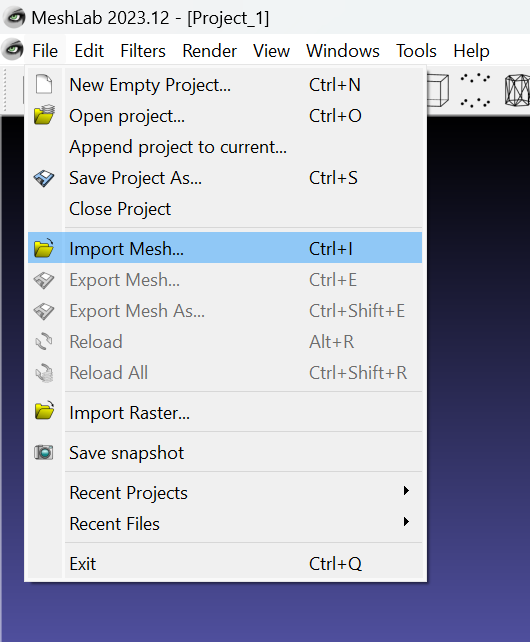
\includegraphics[scale=0.45]{images/importar_01.png}
    \caption{Carga de un archivo de puntos}
\end{figure}

Este es el resultado tras la importación:

\begin{figure}[H]
    \centering
    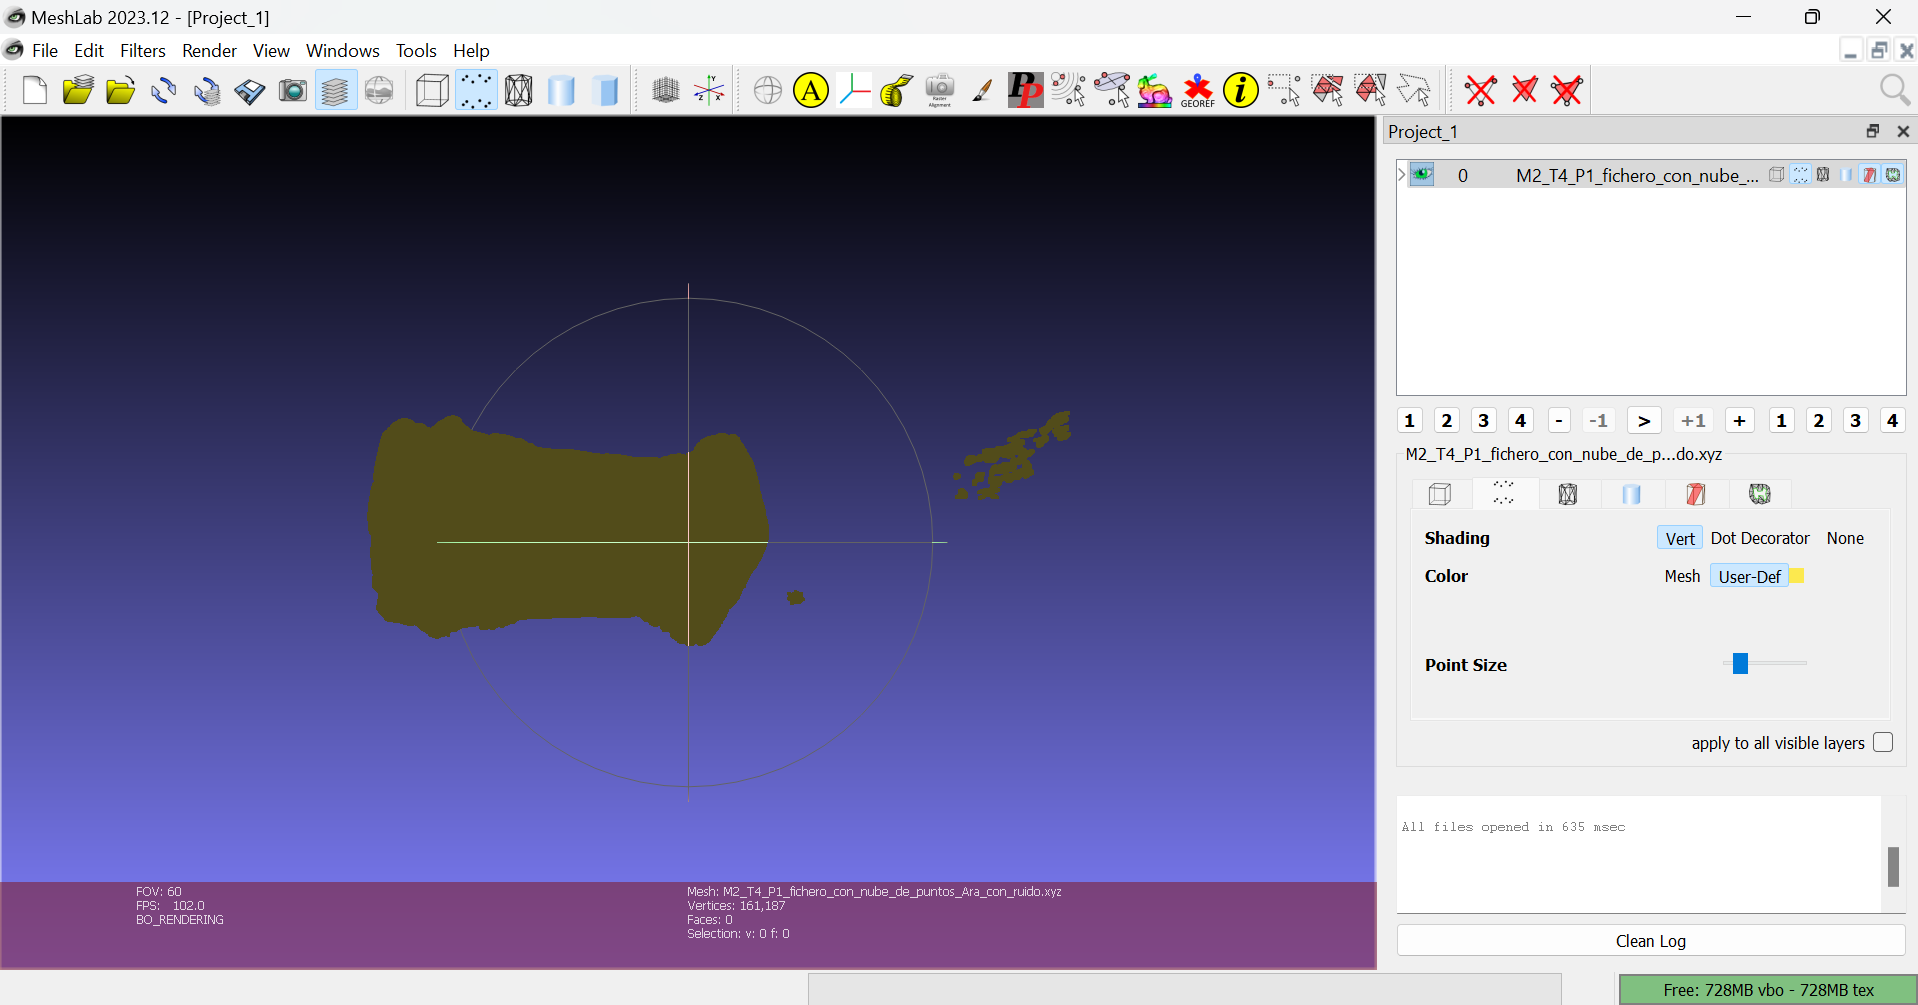
\includegraphics[scale=0.34]{images/importar_02.png}
    \caption{Fichero importado}
\end{figure}

\section{Eliminación del ruido}

Para eliminar el ruido podemos utilizar una herramienta de selección y eliminarlo directamente. Las herramientas de selección y eliminación se encuentran en esta zona del programa:

\begin{figure}[H]
    \centering
    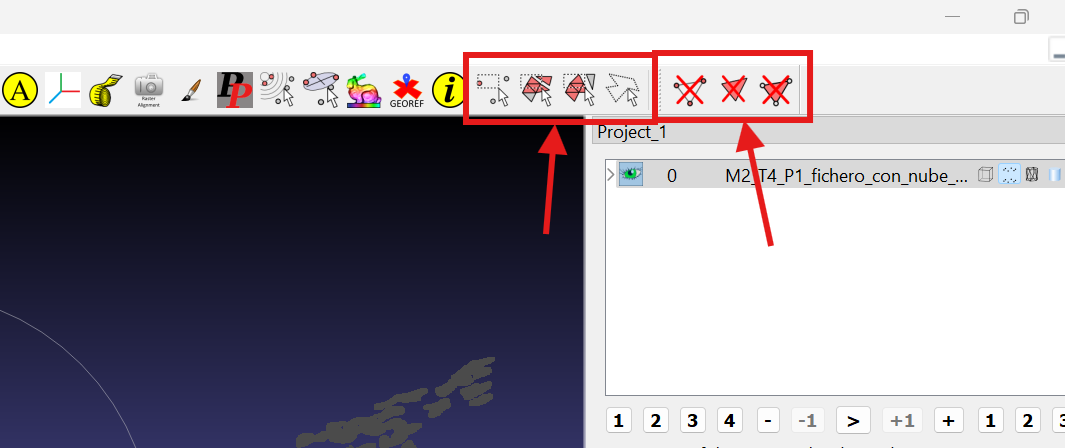
\includegraphics[scale=0.55]{images/ruido_01.png}
    \caption{Selección y borrado}
\end{figure}

\begin{itemize}
    \item El primer rectángulo tiene herramientas de selección
    \item El segundo rectángulo tiene herramientas de borrado
\end{itemize}

\textit{Tip: pasando el puntero por encima te pone qué selecciona y qué borra cada herramienta}

~\\

Para poder trabajar sobre la malla, primero deberemos clonarla. Para ello hacemos \textit{click derecho} sobre ella, y le damos a \textit{``Duplicate current layer''}. Ahora, en nuestro caso, queremos eliminar estas ``nubes'':

\begin{figure}[H]
    \centering
    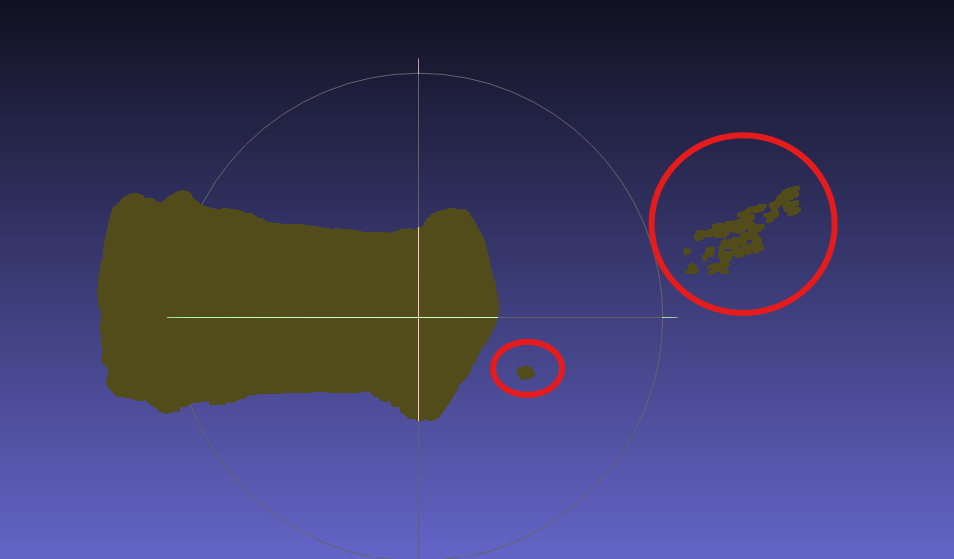
\includegraphics[scale=0.45]{images/ruido_02.png}
    \caption{Ruido que queremos eliminar}
\end{figure}

\pagebreak

Al ser una nube de puntos, deberemos utilizar la \textbf{primera herramienta de selección y borrado} \textit{(select vertices + delete selected vertices)}. El resultado seleccionar y borrar:

\begin{figure}[H]
    \centering
    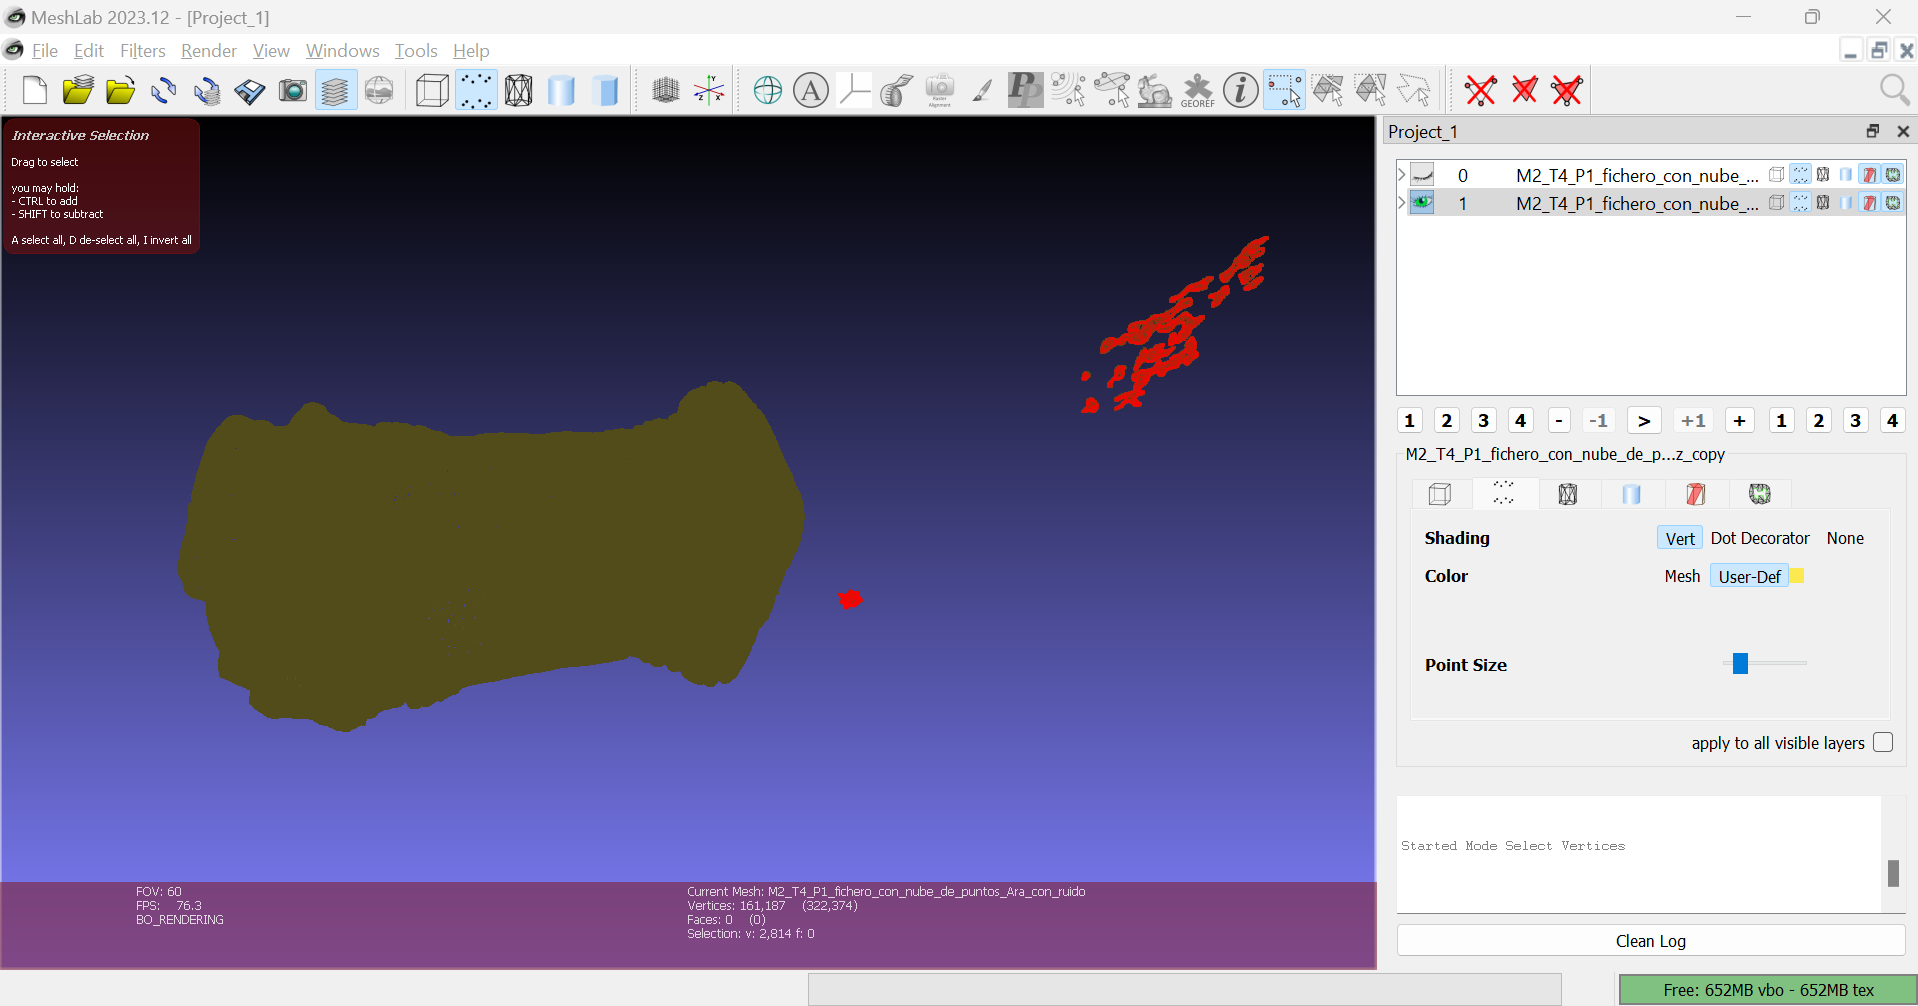
\includegraphics[scale=0.34]{images/ruido_03.png}
    \caption{Ruido seleccionado}
\end{figure}

\begin{figure}[H]
    \centering
    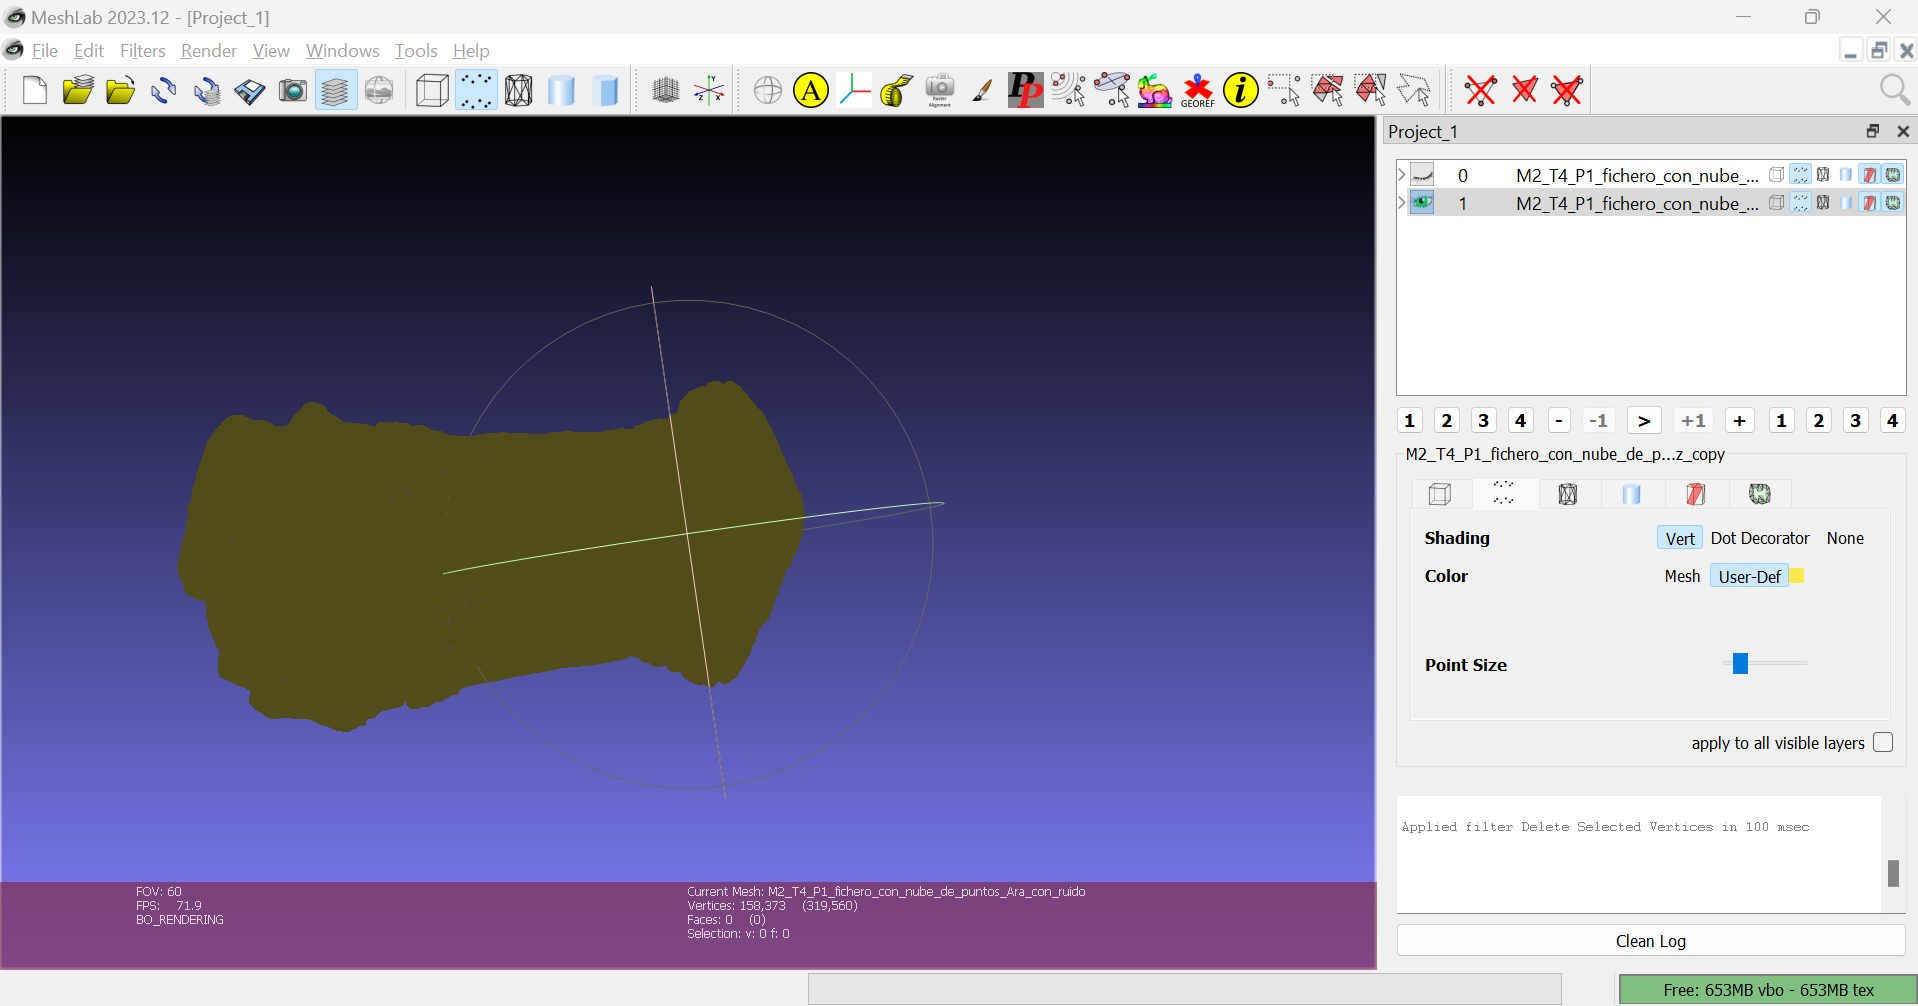
\includegraphics[scale=0.34]{images/ruido_04.png}
    \caption{Ruido borrado}
\end{figure}

\pagebreak

\section{Generación de las normales hacia fuera}

Para calcular las normales de los puntos deberemos hacer click en las siguientes secciones: \textbf{\textit{Filters → Normals, Curvatures and Orientation → Compute normals for pointsets}}:

\begin{figure}[H]
    \centering
    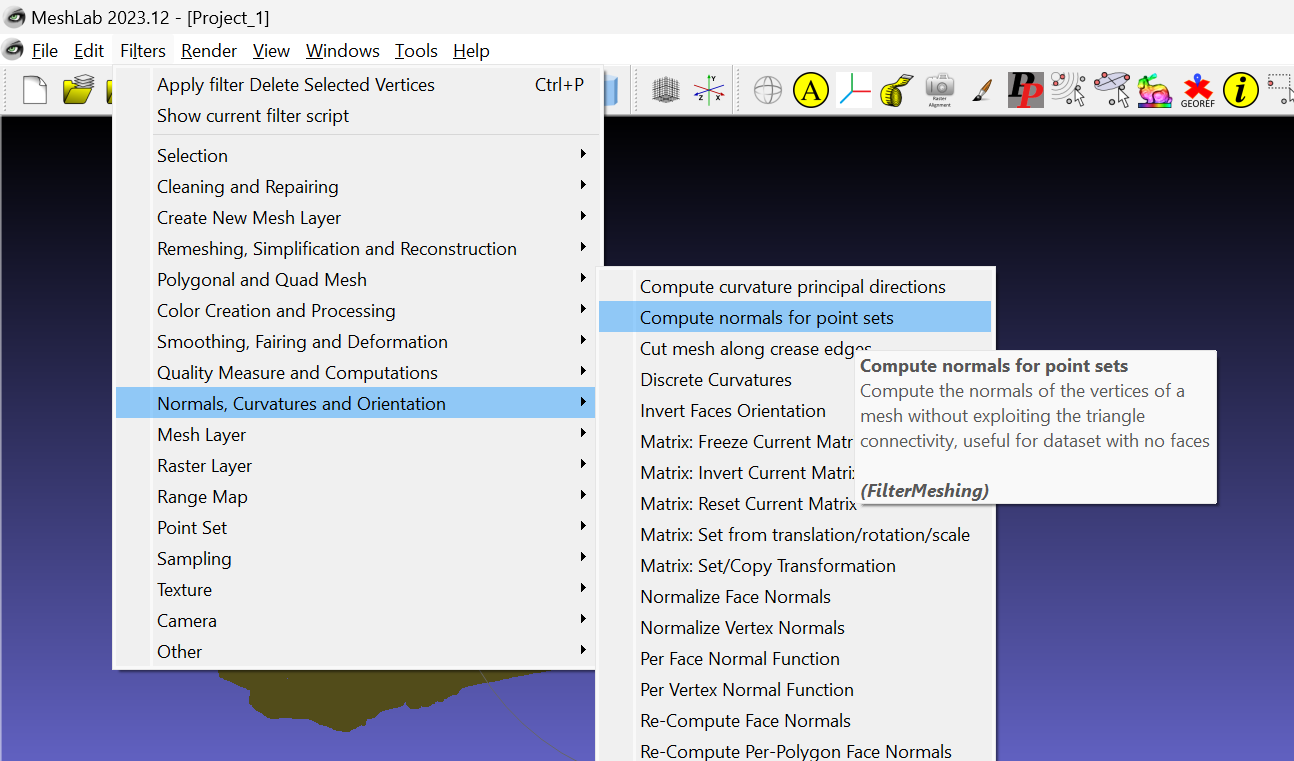
\includegraphics[scale=0.34]{images/normales_01.png}
    \caption{Selección de secciones}
\end{figure}

\end{document}